\documentclass[conference]{IEEEtran}
\usepackage{graphicx,booktabs,amsmath,amssymb,hyperref,placeins,dblfloatfix}
\graphicspath{{./}}
\begin{document}
\title{Cross-Script EEG Identity Recognition During Arabic and Hindi Reading: A Leakage-Conscious Transfer Study}
\author{\IEEEauthorblockN{Author Name}\IEEEauthorblockA{Affiliation\\email}}
\maketitle

\begin{abstract}
We evaluate whether EEG identity information transfers between Arabic- and Hindi-script reading blocks. The analysis uses 296 locally packaged EDF files from 20 adults (10 native Arabic and 10 native Hindi speakers), recorded in one session with a 14-channel scalp montage. Non-overlapping 4-s windows are represented by log and relative band power and band-averaged magnitude-squared coherence. A full language block enrolls each identity and the other block is held out. Data-adaptive preprocessing is fit on enrollment only; the test block is transformed with the frozen procedure. On 20-way identification, the fixed-filter/no-ICA logistic baseline obtains 92.4\% Arabic-to-Hindi and 93.5\% Hindi-to-Arabic balanced accuracy (chance 5\%); enrollment-only ICA sensitivity estimates are 92.8\% and 93.7\%. Cohort-stratified results vary by native-language/nationality group, and four of 20 identities have recall below 90\% in each direction. Because nationality and native language are confounded, sex is imbalanced, block order is fixed, and both blocks come from one session, these results do not establish universal language invariance, longitudinal permanence, or deployable biometric performance. We frame the work as exploratory same-session cross-script identity recognition.
\end{abstract}
\begin{IEEEkeywords}
EEG, biometrics, cross-condition identification, script reading, coherence, evaluation design
\end{IEEEkeywords}

\section{Introduction}
EEG biometric studies show that individuals can be distinguished under a range of recording conditions, while performance may change with task, session, and acquisition protocol~\cite{campisi2014,gui2019,delpozo2018,mota2021}. Mota \emph{et al.} evaluate cross-task identity recognition on motor and motor-imagery EEG~\cite{mota2021}. More directly, Sah \emph{et al.} compare EEG biometrics during native-language songs, non-native-language songs, and neutral music; their IEEE record reports mean sensitivity 96.66\%, specificity 99.82\%, and EER 3.18\%~\cite{sah2025}. These auditory results make language-conditioned identity recognition itself an established topic. The narrower question here is whether identity classification transfers between visual reading blocks using Arabic and Devanagari scripts, including a native-to-foreign script change, with spectral and connectivity representations. The metrics and protocols differ, so the values are not directly comparable.

This is a secondary analysis of a public language-learning dataset, not a new cohort or a deployable system. Our contribution is an audited, within-session transfer protocol and a comparison of power, coherence, their fusion, and compact linear baselines with data-adaptive preprocessing confined to enrollment. The experiment is exploratory: the available recordings couple language with session order, provide only 20 identities, and do not test cross-day stability. We therefore use “cross-script transfer” to describe the measured task and avoid interpreting it as causal language invariance.

\section{Related Work and Research Gap}
\subsection{EEG traits used for person recognition}
EEG biometric research spans ongoing spectral activity, functional connectivity, and stimulus-locked event-related potentials (ERPs). Early statistical and machine-learning systems established that EEG can support person authentication from individual signal features~\cite{marcel2007,palaniappan2007}; subsequent surveys identify acquisition consistency, permanence, task dependence, and evaluation protocol as central challenges~\cite{campisi2014,gui2019}. Most spontaneous-EEG pipelines use spectral power or related features. Connectivity provides complementary information: La Rocca \emph{et al.} evaluated coherence-based networks in resting EEG from 108 participants and found that regional connectivity could distinguish individuals beyond single-channel power in their protocol~\cite{lar2014}. Fraschini \emph{et al.} represented resting EEG as phase-lag-index networks and used eigenvector centrality as a biometric descriptor~\cite{fraschini2015}. These studies motivate testing coherence alongside power here, but their resting-state datasets and splits do not establish cross-script transfer.

ERP biometrics take a different approach by presenting controlled challenges to elicit individual responses. Armstrong \emph{et al.} examined uniqueness and permanence of ERP-based ``Brainprint'' responses~\cite{armstrong2015}; the CEREBRE protocol reported perfect identification in its 50-person cohort under several stimulus configurations~\cite{ruizblondet2016}. Such results demonstrate the value of carefully designed, time-locked stimuli. The present data lack event markers and were not designed as an ERP challenge, so the analysis instead addresses identity information in short-window spectral and connectivity summaries.

\subsection{Task transfer, session permanence, and language}
Task-independent identification and long-term permanence are related but distinct questions. Del Pozo-Ba\~nos \emph{et al.} reported person-specific information in EEG spectral shape that was substantially stable across cognitive tasks and conditions~\cite{delpozo2018}. Wang \emph{et al.} used dynamic functional connectivity and convolutional networks to identify participants across resting and active states~\cite{wang2019}; Maiorana learned deep descriptors for task-independent verification~\cite{maiorana2021}; and Mota \emph{et al.} evaluated cross-task verification on motor and motor-imagery recordings from the 109-participant PhysioNet dataset~\cite{mota2021}. Collectively, this work rules out a claim that cross-task EEG identity recognition is new. It also differs from the present condition: motor imagery and resting/activity changes are not a matched visual-script manipulation, and none of these results should be compared numerically with this 20-person, 14-channel, closed-set experiment because cohorts, protocols, and metrics differ.

Permanence asks whether a template remains useful across sessions separated in time. Maiorana \emph{et al.} assessed three resting-state recordings from 50 participants collected over roughly six weeks~\cite{maiorana2016}; later longitudinal work tested 45 participants across five or six sessions spanning three years~\cite{maiorana2018}. Those studies make clear why same-session transfer cannot establish persistence: electrode placement, impedance, and other session-specific factors can remain shared by the blocks. Our experiment tests only within-session transfer and does not extend that permanence literature.

Language-conditioned EEG biometrics have also been investigated directly in an auditory paradigm. Sah \emph{et al.} compared native-language songs, non-native-language songs, and neutral music using a one-dimensional CNN, reporting mean sensitivity 0.9666, specificity 0.9982, and EER 0.0318~\cite{sah2025}. This study rules out a broad claim that language has not been considered in EEG biometrics. Its auditory/music stimuli and reported verification measures differ from the visual Arabic/Devanagari reading blocks and closed-set identity task here; those scores are therefore contextual rather than directly comparable.

The Arabic--Hindi EEG studies by Aldhaheri \emph{et al.} examine language acquisition, learning-related features, or classification of language-related labels~\cite{aldhaheri2024,aldhaheri2025,aldhaheri2026}. They establish the language-learning context and provide related analyses of this research line, but their prediction target is not participant identity transferred between scripts. Their participant counts and reported dataset descriptions also vary, so these papers should not be assumed to be independent replications or an identical release without a release-level reconciliation. Our contribution is not a new dataset or a new general theory of task-independent EEG identity; it is an audited evaluation of whether identity classification transfers between the two visual script-reading blocks in the locally available Arabic--Hindi recordings, with power/coherence comparisons and enrollment-only fitted preprocessing. Fixed block order, demographic confounding, and the single-session design sharply limit the interpretation of that gap.

\section{Dataset and Task}
The local project package contains 296 EDFs from 20 adults (10 native Arabic speakers and 10 native Hindi speakers), sampled at 256 Hz. The source cohort assigns participants 1--10 to Yemeni/Arabic-native and 11--20 to Indian/Hindi-native groups; project metadata codes 12 participants as male and eight as female, with all ten Arabic-native participants male and the Hindi-native group comprising two male and eight female participants. Native language and nationality are therefore completely confounded, and sex is imbalanced across cohorts. Group analyses below show cohort-specific performance but cannot attribute differences to language, nationality, sex, or physiology separately. We verified that every extracted EDF matches the included raw archive by size and CRC32. This count is four fewer than the 300-file count on the public Mendeley landing page; the local package is analyzed as supplied, and the discrepancy remains unresolved. The dataset and associated language-learning studies are described by Aldhaheri \emph{et al.}~\cite{aldhaheri2024,aldhaheri2025,aldhaheri2026,dataset}.

The same 12 concepts were presented in Arabic and Hindi script. For each participant, one script was native and the other foreign. Files are 56-s EDF chunks; timestamps indicate that Arabic precedes Hindi for all participants, so direction also changes recording time. We retain the 14 scalp electrodes shared across all files and exclude ear-reference and inconsistently present channels. No event markers are available. The task is closed-set 20-way identification: train on all usable windows from one language block and evaluate on the other, then reverse direction. The resulting test set contains 2,198 Hindi windows for Arabic-to-Hindi transfer and 1,946 Arabic windows for Hindi-to-Arabic transfer. Windows are 4 s long, non-overlapping, and never cross an EDF boundary; incomplete final windows are dropped.

\section{Signal Processing and Features}
Each language block is processed separately. The fixed-filter pipeline applies 50/100-Hz notch filtering, a 1--45-Hz band-pass, and common-average reference. Welch power spectral density is computed per window; log and relative power in five frequency bands across 14 channels form 140 features. For connectivity, magnitude-squared coherence is averaged within the same bands for all 91 channel pairs (455 features). The fused representation concatenates power and coherence. Coherence is estimated independently within each 4-s window; no across-window or test-block-fitted connectivity transform is used. Feature scaling and classifier tuning use enrollment windows only.

The primary estimate uses fixed filtering without ICA. In a sensitivity pipeline, FastICA is fit separately for each participant using only the enrollment block, with a 99\% variance criterion. Ocular-correlated component selection uses enrollment-block frontal electrodes only. The frozen decomposition and component list are applied to the test block without refitting. The audit records 40 fits (20 participants by two directions), fit scope, sample counts, exclusions, and channel order. No components were excluded in these runs; consequently the ICA pipeline is a check on fit-scope handling rather than evidence that ocular cleaning improves performance.

We compare standardized multinomial logistic regression, shrinkage LDA, and linear SVM for power features; logistic regression is also used for coherence and fused features. Hyperparameters are selected from the enrollment block only using three folds grouped by EDF file and stratified by participant identity. Scaling is refit within each training fold. The selected model is refit on the complete enrollment block and evaluated once on the opposite-language block.

Figure~\ref{fig:architecture} summarizes the dataset, signal-processing branches, feature representations, and bidirectional evaluation protocol.
\begin{figure*}[t]
\centering
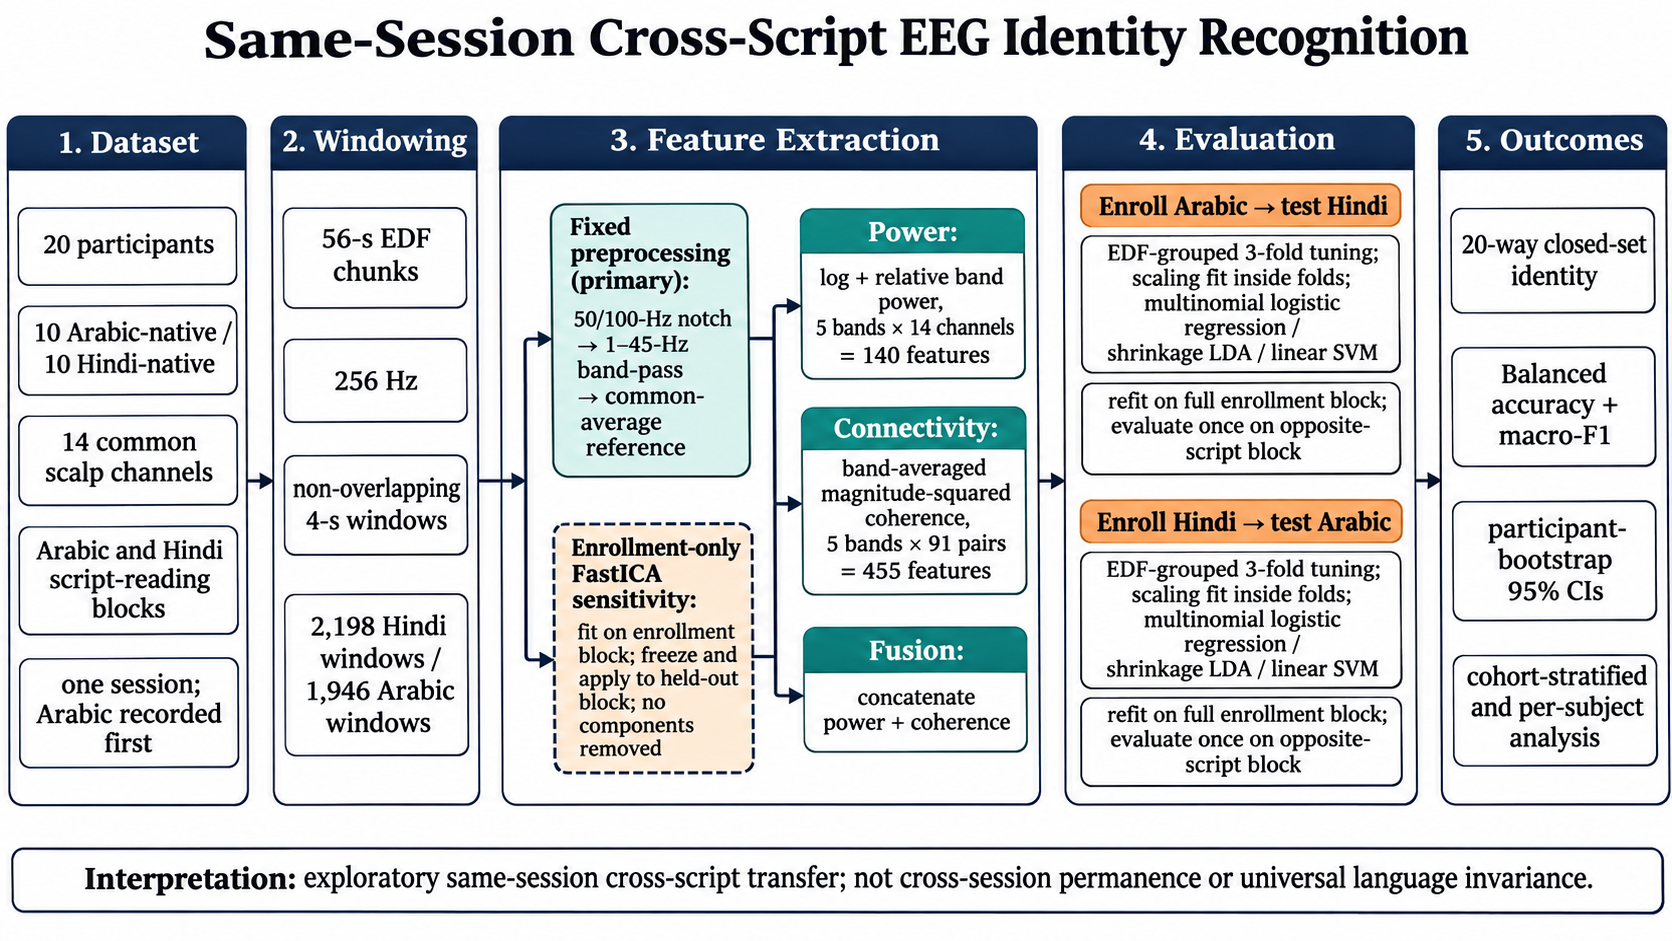
\includegraphics[width=\textwidth]{architecture_cross_script.png}
\caption{Architecture of the same-session cross-script EEG identity-recognition pipeline. The primary analysis uses fixed filtering without ICA; enrollment-only ICA is a sensitivity analysis. The two transfer directions use one script block for enrollment and the opposite-script block for testing.}
\label{fig:architecture}
\end{figure*}

\section{Experimental Design and Statistics}
The primary outcome is 20-way balanced accuracy, equivalent to mean identity recall; we also report macro-F1 over the 20 identity classes. Participant-level precision, recall, and F1 are retained in the per-subject CSV, and normalized confusion matrices are reported separately for both directions. Percentile confidence intervals resample participants—not windows—as the independent units (5,000 resamples for the core model table and 10,000 for macro-F1, demographic and supplementary duration estimates). For the predeclared enrollment-only ICA, power, logistic-regression result in each direction, we permute test identity mappings at participant level 2,000 times; the minimum attainable Monte Carlo p-value is 0.0005. Model contrasts use paired participant recall differences, paired bootstrap intervals, and Wilcoxon signed-rank tests; Holm correction is applied across 12 contrasts.

We vary enrollment size by taking equal numbers of 4-s windows per identity from the training block, averaging ten repeated subsamples at each duration. Separately, test-evidence duration averages logistic posterior scores over consecutive windows within each held-out EDF; uncertainty is computed after aggregation to participant-level recall so multiple segments per person are not treated as independent replicates. These duration analyses remain within-session and do not estimate a real-world enrollment/test-day gap. Frequency/site subsets are sensitivity analyses, not tests that rule out EMG, eye, impedance, or other artifacts. The prior open-set analysis split 20 identities into five groups of four unknowns, trained on the remaining 16, and tested all 20 in the opposite-language block; however, each fold's FPIR threshold was estimated from the same four unknown test identities used to calculate DIR. We therefore exclude those DIR estimates. We also omit the prior posterior-based EER because it lacks independent score calibration and a prespecified claimed-identity trial design. Twenty identities do not support a useful independent enrollment/calibration/final-test cohort.

\section{Results and Limitations}
\begin{table*}[t]
\centering\caption{Primary fixed-filter/no-ICA results and enrollment-only ICA sensitivity results. Entries are participant-bootstrap 95\% CIs; balanced accuracy (BA) chance is 5\%, and macro-F1 is averaged across identities.}
\label{tab:main}\small
\begin{tabular}{lllcccc}\toprule
Features & Model & Preprocessing & Arabic$\to$Hindi BA & Arabic$\to$Hindi F1 & Hindi$\to$Arabic BA & Hindi$\to$Arabic F1\\\midrule
Power & Logistic & No ICA & .924 [.865,.967] & .918 [.879,.949] & .935 [.889,.967] & .934 [.905,.956]\\
Power + coherence & Logistic & No ICA & .960 [.932,.983] & .960 [.943,.974] & .964 [.920,.990] & .962 [.934,.982]\\
Power & Logistic & ICA (enroll.) & .928 [.872,.968] & .922 [.885,.951] & .937 [.892,.968] & .935 [.907,.957]\\
Power & Shrinkage LDA & ICA (enroll.) & .895 [.813,.961] & .882 [.819,.936] & .942 [.895,.977] & .940 [.913,.964]\\
Power & Linear SVM & ICA (enroll.) & .951 [.918,.977] & .948 [.926,.965] & .946 [.901,.977] & .944 [.915,.966]\\
Coherence & Logistic & ICA (enroll.) & .950 [.923,.972] & .949 [.932,.965] & .957 [.910,.985] & .955 [.925,.976]\\
Power + coherence & Logistic & ICA (enroll.) & .958 [.929,.980] & .957 [.940,.973] & .962 [.916,.989] & .959 [.931,.978]\\\bottomrule
\end{tabular}
\end{table*}

\begin{table*}[t]
\centering\caption{Primary enrollment-only ICA power/logistic performance by native-language cohort. Each cohort has 10 participants; entries show mean participant recall (BA) and macro-F1 with participant-bootstrap 95\% CIs.}
\label{tab:cohort}\small
\begin{tabular}{lccccc}\toprule
Direction & Arabic-native BA & Arabic-native F1 & Hindi-native BA & Hindi-native F1 & BA gap (Arabic$-$Hindi)\\\midrule
Arabic$\to$Hindi & .971 [.954,.985] & .939 [.906,.965] & .885 [.785,.962] & .905 [.840,.954] & .086 [.008,.188]\\
Hindi$\to$Arabic & .961 [.936,.980] & .958 [.943,.972] & .913 [.832,.972] & .913 [.866,.952] & .047 [$-$.017,.132]\\\bottomrule
\end{tabular}
\end{table*}

The filtered no-ICA logistic baseline reaches 92.4\% and 93.5\% using power, and 96.0\% and 96.4\% with fused features. Thus the enrollment-only ICA estimates are similar; ICA does not materially raise the primary logistic power result. Participant-level permutation tests for the two enrollment-only ICA power results both yield $p=0.0005$ at the 2,000-permutation resolution. This rejects chance-level identity mapping under this protocol, not broader claims about what signal carries identity. The largest results are fused-feature estimates; participant-paired recall differences were not significant after Holm correction across 12 model/preprocessing contrasts (minimum adjusted $p=.077$), so we do not claim a reliable representation or classifier ranking.

Three-fold file-level validation within the enrollment block gives 98.0\% and 98.6\% balanced accuracy for logistic power, about five percentage points above cross-block test performance. This gap indicates that validation within a language block does not fully predict transfer to the other block and supports treating the held-out cross-script evaluation as the relevant result. For the fixed-filter/no-ICA primary model, macro-F1 is 91.8\% [87.9, 94.9] and 93.4\% [90.5, 95.6] in the two directions (Table~\ref{tab:main}).

Arabic-native participants have higher mean recall than Hindi-native participants in both directions (Table~\ref{tab:cohort}); the gap is 8.6 points for Arabic-to-Hindi and 4.7 points for Hindi-to-Arabic, with substantial uncertainty. Because cohort is confounded with nationality and sex, this analysis cannot determine which group characteristic explains the difference. Sex-stratified recall is 96.3\% [93.9, 98.3] for 12 male-coded and 87.5\% [75.1, 96.6] for eight female-coded participants in Arabic-to-Hindi, and 93.1\% [86.2, 97.5] and 94.6\% [90.9, 98.1] in Hindi-to-Arabic. Individual recall ranges from 50.0\% to 100\% and 59.2\% to 100\%, respectively; two and one participants fall below 80\% recall. These results show substantial between-person heterogeneity despite high aggregate scores.

Figure~\ref{fig:transfer} summarizes the cross-script transfer estimates across the tested representations.
\begin{figure}[!htbp]\centering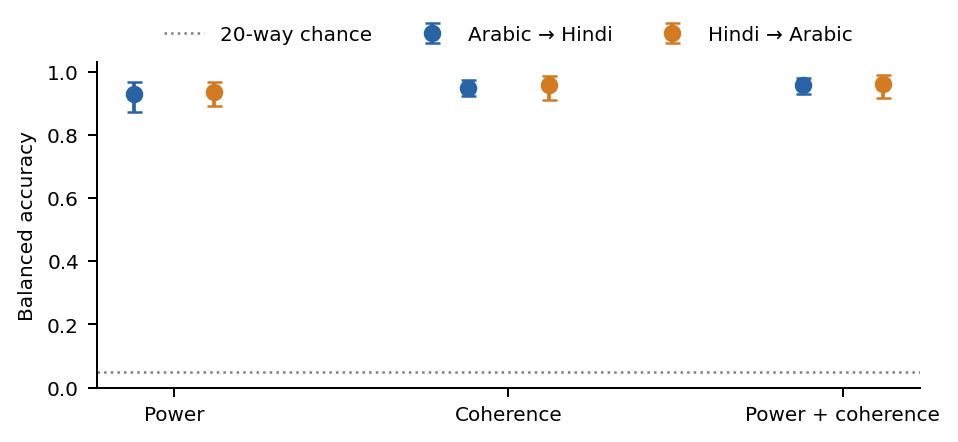
\includegraphics[width=.96\columnwidth]{transfer_results.png}\caption{Enrollment-only ICA transfer accuracy by representation; bars show participant-bootstrap 95\% intervals.}\label{fig:transfer}\end{figure}

Figure~\ref{fig:confusion} shows the per-identity error patterns for both transfer directions.
\begin{figure*}[!tb]\centering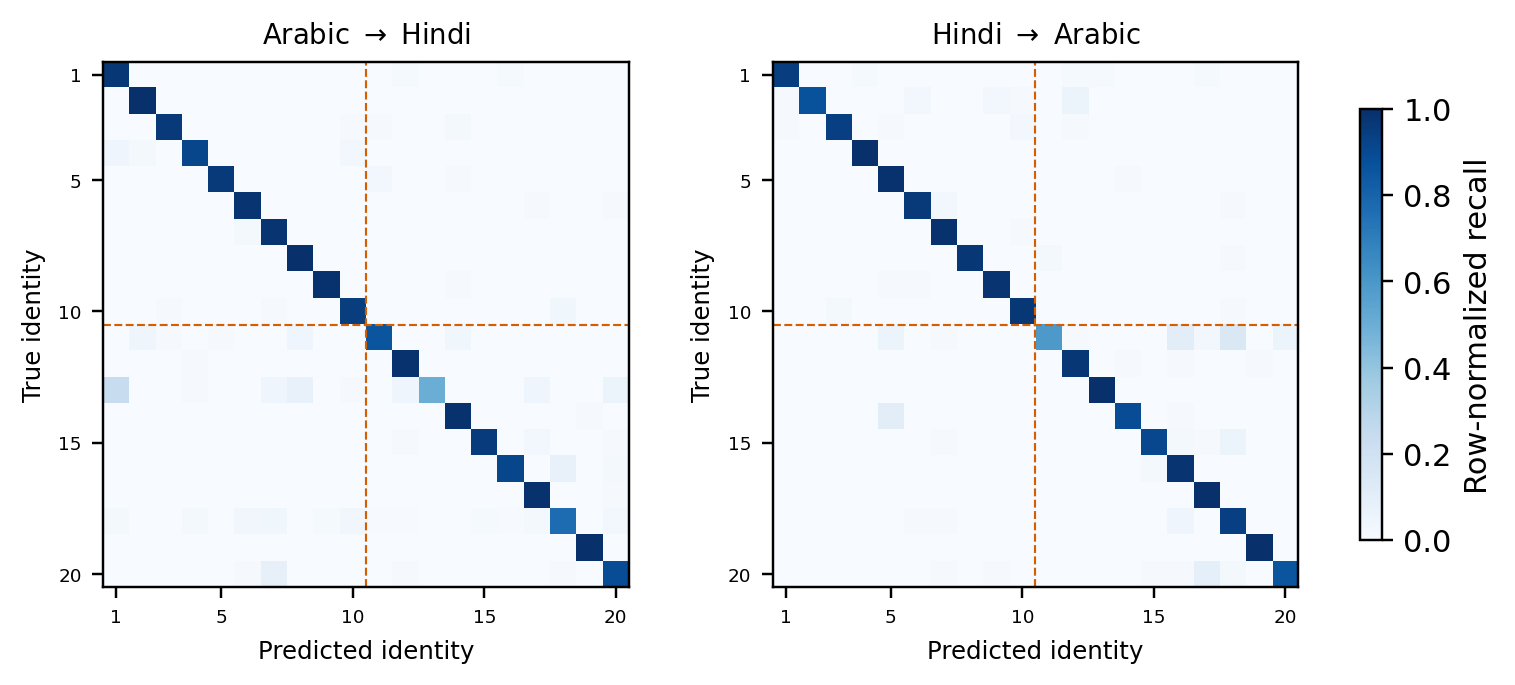
\includegraphics[width=.72\textwidth]{confusion_primary_directions.png}\caption{Separate row-normalized confusion matrices for the enrollment-only ICA power/logistic model. Dashed lines separate IDs 1--10 (Arabic-native/Yemeni) and 11--20 (Hindi-native/Indian) cohorts. Per-identity matrices are supplied as CSV.}\label{fig:confusion}\end{figure*}

With enrollment-only ICA and power, aggregating test scores across 16 s gives 96.4\% [90.7, 99.5] and 96.8\% [93.4, 99.2], and across 32 s gives 97.9\% [93.6, 100] and 97.5\% [93.6, 100] for Arabic-to-Hindi and Hindi-to-Arabic, respectively; intervals bootstrap participants after within-person aggregation. Enrollment duration is a distinct constraint: at one 4-s window per identity, mean accuracy is 54.1\% and 53.7\%; at 32 windows (128 s per identity) it is 89.2\% and 92.0\%. The apparent saturation near full enrollment highlights the cost of enrollment data and the difference between test aggregation and template training.
Figure~\ref{fig:duration} summarizes how enrollment size and accumulated test evidence affect the measured accuracy.
\begin{figure}[!htbp]\centering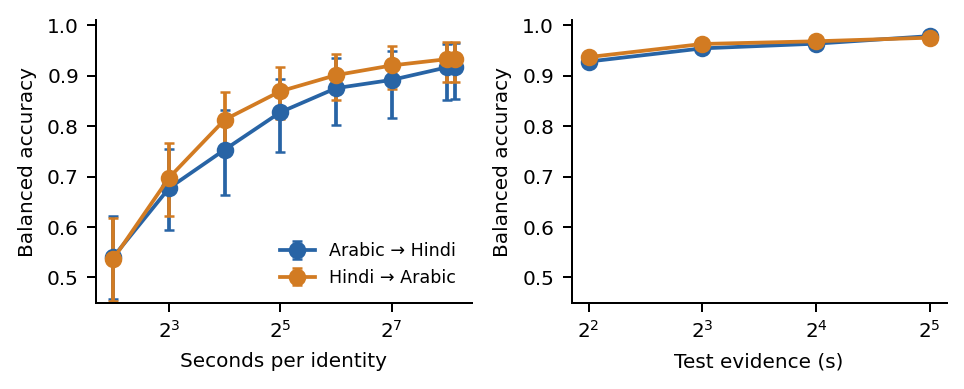
\includegraphics[width=.96\columnwidth]{duration_results.png}\caption{Descriptive enrollment-size (left, participant-bootstrap intervals) and test-evidence (right) curves using enrollment-only ICA and power/logistic regression.}\label{fig:duration}\end{figure}

Restricting to 1--13-Hz power at all channels yields 87.5\% and 90.7\%; restricting further to six posterior/frontal sites yields 76.1\% and 74.9\%. This shows that above-chance identity information persists under restricted frequency/channel conditions, while performance decreases. It does not rule out muscle contamination or establish that the remaining signal is neural. The core limitation is design confounding: Arabic is always recorded before Hindi, so language, fatigue, adaptation, and time are inseparable. Both blocks are from one session; no long-term biometric permanence or cross-session generalization is demonstrated. Further limits are only 20 participants, unequal available files/windows, cohort/demographic confounding, uncertain archive-version discrepancy, no independent external cohort, and pending target-venue page-fit and final PDF layout checks. The direct auditory-language biometric study~\cite{sah2025} also limits novelty to this particular visual script-transfer setting. Cross-study accuracy is not compared numerically because modalities, cohorts, splits, and metrics differ.

Under the same file-level tuning and classifier protocol, historical features generated by fitting ICA on concatenated enrollment and test blocks yield 93.1\% [87.5, 97.2] and 94.6\% [90.1, 97.6], versus 92.8\% and 93.7\% with enrollment-only ICA. This is test-distribution exposure, although identity labels from the test block are not used to fit ICA. Paired participant differences (enrollment-only minus full-session) are $-0.3$ and $-0.9$ points (Holm-adjusted $p=.685$ and $.578$). This matched diagnostic does not show that test-distribution exposure is harmless; it shows that correcting the fit scope did not materially change these point estimates in this cohort.

\section{Conclusion}
In this local 20-person dataset, a model trained on one script-reading block identifies participants above chance in the other block, with 92.4--93.7\% power-based balanced accuracy across the fixed-filter primary and enrollment-only ICA analyses. Cohort-stratified and per-person results show heterogeneity, while native language, nationality, and sex cannot be isolated in this sample. These findings support cross-script transfer as an evaluation condition, not universal language invariance or a language-invariant neural biometric claim. A stronger study requires counterbalanced script order, more diverse identities, repeated sessions, independent cohort-level calibration, direct ocular/EMG controls, and preregistered external testing. The present results and provenance audit should be treated as exploratory pending those tests.

% Keep pending IEEE floats with the paper body, before the references.
\FloatBarrier
\begin{thebibliography}{99}
\bibitem{campisi2014} P. Campisi and D. La Rocca, ``Brain waves for automatic biometric-based user recognition,'' \emph{IEEE Trans. Inf. Forensics Security}, vol. 9, no. 5, pp. 782--800, 2014, doi:10.1109/TIFS.2014.2308640.
\bibitem{gui2019} Q. Gui \emph{et al.}, ``A survey on brain biometrics,'' \emph{ACM Comput. Surv.}, vol. 51, no. 6, art. 112, 2019, doi:10.1145/3230632.
\bibitem{delpozo2018} M. del Pozo-Ba\~nos \emph{et al.}, ``Evidence of a task-independent neural signature in the spectral shape of the electroencephalogram,'' \emph{Int. J. Neural Syst.}, vol. 28, no. 1, 1750035, 2018, doi:10.1142/S0129065717500356.
\bibitem{mota2021} M. R. F. Mota \emph{et al.}, ``A deep descriptor for cross-tasking EEG-based recognition,'' \emph{PeerJ Comput. Sci.}, vol. 7, e549, 2021, doi:10.7717/peerj-cs.549.
\bibitem{sah2025} A. Sah, A. Ahirwal, and G. S. Tomar, ``Deep learning and EEG signal based biometric system: An application of brain computer interface,'' in \emph{Proc. IEEE SCEECS}, 2025, doi:10.1109/SCEECS64059.2025.10940880.
\bibitem{marcel2007} S. Marcel and J. d. R. Mill\'an, ``Person authentication using brainwaves (EEG) and maximum a posteriori model adaptation,'' \emph{IEEE Trans. Pattern Anal. Mach. Intell.}, vol. 29, no. 4, pp. 743--752, 2007, doi:10.1109/TPAMI.2007.1012.
\bibitem{palaniappan2007} R. Palaniappan and D. P. Mandic, ``Biometrics from brain electrical activity: A machine learning approach,'' \emph{IEEE Trans. Pattern Anal. Mach. Intell.}, vol. 29, no. 4, pp. 738--742, 2007, doi:10.1109/TPAMI.2007.1013.
\bibitem{lar2014} D. La Rocca \emph{et al.}, ``Human brain distinctiveness based on EEG spectral coherence connectivity,'' \emph{IEEE Trans. Biomed. Eng.}, vol. 61, no. 9, pp. 2406--2412, 2014, doi:10.1109/TBME.2014.2317881.
\bibitem{fraschini2015} M. Fraschini, A. Hillebrand, M. Demuru, L. Didaci, and G. L. Marcialis, ``An EEG-based biometric system using eigenvector centrality in resting state brain networks,'' \emph{IEEE Signal Process. Lett.}, vol. 22, no. 6, pp. 666--670, 2015, doi:10.1109/LSP.2014.2367091.
\bibitem{armstrong2015} B. C. Armstrong \emph{et al.}, ``Brainprint: Assessing the uniqueness, collectability, and permanence of a novel method for ERP biometrics,'' \emph{Neurocomputing}, vol. 166, pp. 59--67, 2015, doi:10.1016/j.neucom.2015.04.025.
\bibitem{ruizblondet2016} M. V. Ruiz-Blondet, Z. Jin, and S. Laszlo, ``CEREBRE: A novel method for very high accuracy event-related potential biometric identification,'' \emph{IEEE Trans. Inf. Forensics Security}, vol. 11, no. 7, pp. 1618--1629, 2016, doi:10.1109/TIFS.2016.2543524.
\bibitem{wang2019} M. Wang, H. El-Fiqi, J. Hu, and H. A. Abbass, ``Convolutional neural networks using dynamic functional connectivity for EEG-based person identification in diverse human states,'' \emph{IEEE Trans. Inf. Forensics Security}, vol. 14, no. 12, pp. 3259--3272, 2019, doi:10.1109/TIFS.2019.2916403.
\bibitem{maiorana2021} E. Maiorana, ``Learning deep features for task-independent EEG-based biometric verification,'' \emph{Pattern Recognit. Lett.}, vol. 143, pp. 122--129, 2021, doi:10.1016/j.patrec.2021.01.004.
\bibitem{maiorana2016} E. Maiorana, D. La Rocca, and P. Campisi, ``On the permanence of EEG signals for biometric recognition,'' \emph{IEEE Trans. Inf. Forensics Security}, vol. 11, no. 1, pp. 163--175, 2016, doi:10.1109/TIFS.2015.2481870.
\bibitem{maiorana2018} E. Maiorana and P. Campisi, ``Longitudinal evaluation of EEG-based biometric recognition,'' \emph{IEEE Trans. Inf. Forensics Security}, vol. 13, no. 5, pp. 1123--1138, 2018, doi:10.1109/TIFS.2017.2778010.
\bibitem{aldhaheri2024} T. A. Aldhaheri \emph{et al.}, ``Investigation of brain response to acquisition and learning the second languages based on EEG signals and machine learning techniques,'' \emph{Cogent Arts Humanit.}, vol. 11, no. 1, 2416759, 2024, doi:10.1080/23311983.2024.2416759.
\bibitem{aldhaheri2025} T. A. Aldhaheri \emph{et al.}, ``Utilizing machine and deep learning algorithms to identify learning-related features in electroencephalography data during second language acquisition,'' \emph{Cogent Arts Humanit.}, vol. 12, no. 1, 2025, doi:10.1080/23311983.2025.2485696.
\bibitem{aldhaheri2026} T. A. Aldhaheri \emph{et al.}, ``Optimizing machine learning models with multi feature selection for EEG analysis in second language acquisition research,'' \emph{Discover Artif. Intell.}, vol. 6, art. 99, 2026, doi:10.1007/s44163-025-00801-z.
\bibitem{dataset} T. A. Aldhaheri, S. B. Kulkarni, and M. Tawfik, ``EEG dataset for second language acquisition Arabic and Hindi,'' Mendeley Data, V1, 2026, doi:10.17632/7cdyp2r5cz.1.
\end{thebibliography}
\end{document}
